%%%===========HỘP BÀI TẬP TRẮC NGHIỆM TỰ LUẬN=================%%%
\newcommand\circl[2][\mycolor]{\tikz[baseline=(char.base)]{\node[shape=circle,inner sep=1pt,draw=#1,fill=#1!15,font=\fontfamily{qag}\selectfont,minimum size=15pt] (char) {\color{\mycolor!50!black}\bfseries%
			#2};}}
\usepackage{ex_test}
\usepackage{ifthen}
\renewcommand{\FalseEX}{\stepcounter{dapan}{\circl{\Alph{dapan}}}}
\renewcommand{\TrueEX}{\stepcounter{dapan}{\circl{\Alph{dapan}}}}

\renewcommand{\immini}[3][]{%
	\tcbsidebyside[
	sidebyside adapt=right,
	blanker,sidebyside gap=5mm,
	sidebyside align=top seam
	]{%
		#2
	}{%
		#3
	}
}
\renewcommand{\hinhphai}[2]{%
	\tcbsidebyside[
	sidebyside adapt=right,
	blanker,sidebyside gap=3mm,
	sidebyside align=top seam,
	]{%
		#1
	}{%
		#2
	}
}
%%%%%%%%%%%%%%%%%%%%%%Tách lời giải%%%%%%%%%%%%%%%%%%%%%%%%%%%%%%%%%%%%%%%%
\Newassociation{giaibt}{loigiaibt}{ansbt}
\Newassociation{giaiex}{loigiaiex}{ansex}
\NewTColorBox{ansbt}{m}{
	breakable,
	enhanced,
	outer arc=0pt,
	arc=0pt,
	colframe=white,
	frame hidden,
	left=-6pt,right=0pt,top=0pt,
	colback=white,
	attach boxed title to top left,
	boxed title style={
		colback=white,
		outer arc=0pt,
		arc=0pt,
		top=1pt,
		bottom=1pt,
		left=3pt,
		right=3pt,
		colframe=white
	},
	fonttitle=\bfseries\sffamily\selectfont\color{white},
	title={HDBT~#1},
	overlay unbroken and first={
		\path (title.north west) coordinate (A)
		($ (title.south west) +(-4pt,0pt)$) coordinate (B)
		(title.south east) coordinate (C)
		($ (title.north east)+(4pt,0) $) coordinate (D);
		\path[rounded corners=2pt,fill=\mycolor,
		preaction={transform canvas={shift={(-45:2pt)}},left color=\mycolor!45,right color=\mycolor!25}] 
		(A)--(B)--(C)--(D)--cycle;
		\path (A)--(C) node[midway,font=\color{white}\bfseries\sffamily\selectfont](Bai){\textsl{HDBT~#1}};
		\draw[rounded corners=2pt,thick,\mycolor] ([xshift=-3pt]B) coordinate (Bt)
		--([shift={(-2pt,2pt)}]A)--+(\linewidth,0) coordinate (Ct);
		\fill[\mycolor] (Bt) circle (1pt) (Ct) circle (2pt);
	}
}

\NewTColorBox{ansex}{m}{
	breakable,
	enhanced,
	outer arc=0pt,
	arc=0pt,
	colframe=white,
	frame hidden,
	left=-6pt,right=0pt,top=0pt,
	colback=white,
	attach boxed title to top left,
	boxed title style={
		colback=white,
		outer arc=0pt,
		arc=0pt,
		top=1pt,
		bottom=1pt,
		left=3pt,
		right=3pt,
		colframe=white
	},
	fonttitle=\bfseries\sffamily\selectfont\color{white},
	title={HD Câu~#1},
	overlay unbroken and first={
		\path (title.north west) coordinate (A)
		($ (title.south west) +(-4pt,0pt)$) coordinate (B)
		(title.south east) coordinate (C)
		($ (title.north east)+(4pt,0) $) coordinate (D);
		\path[rounded corners=2pt,fill=\mycolor,
		preaction={transform canvas={shift={(-45:2pt)}},left color=\mycolor!45,right color=\mycolor!25}] 
		(A)--(B)--(C)--(D)--cycle;
		\path (A)--(C) node[midway,font=\color{white}\bfseries\sffamily\selectfont](Bai){\textsl{HD Câu~#1}};
		\draw[rounded corners=2pt,thick,\mycolor] ([xshift=-3pt]B) coordinate (Bt)
		--([shift={(-2pt,2pt)}]A)--+(\linewidth,0) coordinate (Ct);
		\fill[\mycolor] (Bt) circle (1pt) (Ct) circle (2pt);
	}
}
\def\ansexhead{\begin{ansex}}
\def\ansexend{\end{ansex}}
\renewenvironment{loigiaibt}[1]{\begin{ansbt}{#1}}{\end{ansbt}}
\renewenvironment{loigiaiex}[1]{\ansexhead{#1}}{\ansexend}
\def\luuloigiaibt{
		\AtBeginEnvironment{bt}{
				\renewcommand{\loigiai}[1]{%
				\end{btbox}
				\def\btend{}
					\scantokens{%
							\begin{giaibt}
									##1
							\end{giaibt}}
				}
		}
}
\def\luuloigiaiex{
	\AtBeginEnvironment{ex}{
		\renewcommand{\loigiai}[1]{%
			\ifnum\the\value{numTrue}=1
			\scantokens{%
				\begin{giaiex}
					##1
					\phantom{a}\hfill{\bfseries\sffamily Chọn~\circleTrue{A}}
			\end{giaiex}}
			\fi%
			\ifnum\the\value{numTrue}=2
			\scantokens{%
				\begin{giaiex}
					##1
					\phantom{a}\hfill{\bfseries\sffamily Chọn~\circleTrue{B}}
			\end{giaiex}}
			\fi%	    
			\ifnum\the\value{numTrue}=3
			\scantokens{%
				\begin{giaiex}
					##1
					\phantom{a}\hfill{\bfseries\sffamily Chọn~\circleTrue{C}}
				\end{giaiex}}
			\fi  %	   
			\ifnum\the\value{numTrue}=4
			\scantokens{%
				\begin{giaiex}
					##1
					\phantom{a}\hfill{\bfseries\sffamily Chọn~\circleTrue{D}}
				\end{giaiex}}
			\fi  
		}  
	}
}

%%%%%%%%%%%%%%%%%%%%%%%%%%%%%%%%%%%%%%%%%%%%%%%%%%%%%%%%%%%%%%%%%%%%%%%%%%%%%%%
%%%%%%%%%%%%%%%%%%%%%%%%%%%%%%%%HỘP CÂU CÓ 3 TÙY CHỌN%%%%%%%%%%%%%%%%%%%%%%%%%%%%%
\newbool{ktex}
\newcommand{\sodongkeex}[1][]{\global\setbool{ktex}{true}\end{exbox}\def\exend{} \noindent\textcolor{\mycolor}{\reflectbox{\Large\WritingHand}\ {\fmmfamily\LARGE Bài làm:}}\taodongke{#1}}
%\newcounter{ex}
\NewTColorBox[auto counter]{exbox}{+!O{}O{}O{}}{%
enhanced,
breakable,
fonttitle=\bfseries\sffamily\color{white},
title={\faClockO\ Câu~\theex},
colframe=\mycolor!65!black,
colback=white,
colbacktitle=white,
fonttitle=\bfseries,
coltitle=black,
attach boxed title to top left=
{yshift=-2mm-\tcboxedtitleheight,yshifttext=2mm-\tcboxedtitleheight/2},
boxed title style={
	frame hidden,
	outer arc=0pt,
	arc=0pt,
	top=3pt,
	bottom=3pt,
	left=0pt,
	right=0pt
},
overlay unbroken ={
	\path
	($ (title.north west) +(-2pt,0pt)$) coordinate (A)
	($ (title.south west) +(-2pt,3pt)$) coordinate (B)
	($ (title.south east)+(3pt,3pt) $) coordinate (C)
	($ (title.north east)+(3pt,0) $) coordinate (D)
	($ (A)+(0.99*\linewidth,0) $) coordinate (E)
	;
	\path[fill=\mycolor!15,rounded corners=3pt]
	(A)--(B)--([xshift=0.85*\linewidth]C) coordinate (E)--([xshift=0.85*\linewidth]D) coordinate (F)--cycle;
	\path[fill=\mycolor!70!black,rounded corners=2pt]
	(A)--(B)--([xshift=3pt]C)--([xshift=3pt]D)--cycle;
	\path[left color=\mycolor,right color=\mycolor,rounded corners=3pt]
	([xshift=-2pt]A)--([xshift=-2pt]B)--(C)--(D)--cycle;
	\path ($ (A)!0.5!(B) +(0pt,0)$) node[anchor=west,font=\color{white}\bfseries\sffamily\selectfont]{{\faClockO\ Câu~\theex}};
	\path ($ (C)!0.5!(D) +(9pt,0)$) node[anchor=west,font=\color{\mycolor}]{\taosao{#2}};
	\path ($ (E)!0.5!(F) +(-9pt,0)$) node[anchor=east,font=\color{\mycolor!70!black}\itshape\bfseries]{#1};
	\path ([shift={(-1pt,7pt)}]frame.south east) node[anchor=east,font=\fontsize{9.2 pt}{1pt}\selectfont\color{\mycolor!70!black}\itshape\bfseries]{#3};
},
overlay first={
	\path
	($ (title.north west) +(-2pt,0pt)$) coordinate (A)
	($ (title.south west) +(-2pt,3pt)$) coordinate (B)
	($ (title.south east)+(3pt,3pt) $) coordinate (C)
	($ (title.north east)+(3pt,0) $) coordinate (D)
	($ (A)+(0.99*\linewidth,0) $) coordinate (E)
	;
	\path[fill=\mycolor!15,rounded corners=3pt]
	(A)--(B)--([xshift=0.85*\linewidth]C) coordinate (E)--([xshift=0.85*\linewidth]D) coordinate (F)--cycle;
	\path[fill=\mycolor!70!black,rounded corners=2pt]
	(A)--(B)--([xshift=3pt]C)--([xshift=3pt]D)--cycle;
	\path[left color=\mycolor,right color=\mycolor,rounded corners=3pt]
	([xshift=-2pt]A)--([xshift=-2pt]B)--(C)--(D)--cycle;
	\path ($ (A)!0.5!(B) +(0pt,0)$) node[anchor=west,font=\color{white}\bfseries\sffamily\selectfont]{{\faClockO\ Câu~\theex}};
	\path ($ (C)!0.5!(D) +(9pt,0)$) node[anchor=west,font=\color{\mycolor}]{\taosao{#2}};
	\path ($ (E)!0.5!(F) +(-9pt,0)$) node[anchor=east,font=\color{\mycolor!70!black}\itshape\bfseries]{#1};
},
overlay middle ={
	\path
	($ (title.north west) +(-2pt,0pt)$) coordinate (A)
	($ (title.south west) +(-2pt,3pt)$) coordinate (B)
	($ (title.south east)+(3pt,3pt) $) coordinate (C)
	($ (title.north east)+(3pt,0) $) coordinate (D)
	($ (A)+(0.99*\linewidth,0) $) coordinate (E)
	;
	\path(A)--(B)--([xshift=0.85*\linewidth]C) coordinate (E)--([xshift=0.85*\linewidth]D) coordinate (F)--cycle;
	\path(A)--(B)--([xshift=3pt]C)--([xshift=3pt]D)--cycle;
},
overlay  last ={
	\path
	($ (title.north west) +(-2pt,0pt)$) coordinate (A)
	($ (title.south west) +(-2pt,3pt)$) coordinate (B)
	($ (title.south east)+(3pt,3pt) $) coordinate (C)
	($ (title.north east)+(3pt,0) $) coordinate (D)
	($ (A)+(0.99*\linewidth,0) $) coordinate (E)
	;
	\path(A)--(B)--([xshift=0.85*\linewidth]C) coordinate (E)--([xshift=0.85*\linewidth]D) coordinate (F)--cycle;
	\path(A)--(B)--([xshift=3pt]C)--([xshift=3pt]D)--cycle;
	\path ([shift={(-1pt,7pt)}]frame.south east) node[anchor=east,font=\fontsize{9.2 pt}{1pt}\selectfont\color{\mycolor!70!black}\itshape\bfseries]{#3};
},
top=\tcboxedtitleheight
}
\def\exhead#1#2#3{\begin{exbox}[#1][#2][#3]}
\def\exend{\end{exbox}}
\RenewDocumentEnvironment{ex}{+!O{}O{}O{}}{
\ifblank{#1}{\def\tuychonone{}}{\def\tuychonone{#1}}
\ifblank{#2}{\def\tuychontwo{0}}{\def\tuychontwo{#2}}
\ifblank{#3}{\def\tuychonthree{}}{\def\tuychonthree{#3}}
\exhead{\tuychonone}{\tuychontwo}{\tuychonthree}
}{\exend}
\AtBeginEnvironment{ex}{%
\renewcommand{\FalseEX}{\stepcounter{dapan}{\circl{\Alph{dapan}}}}
\renewcommand{\TrueEX}{\stepcounter{dapan}{\circl{\Alph{dapan}}}}
\refstepcounter{ex} % tăng số điếm bt lên 1
\global\setbool{ktex}{false}
\setcounter{numTrue}{0}%
\setcounter{numTrueSol}{0}%
\renewcommand{\loigiai}[1]{%
	\ifbool{ktex}{}{
	\end{exbox}
	\def\exend{}
	%%==================Tính số dòng của lời giải==================%%%
	\setbox0=\vbox{\hbox{
			\noindent\begin{minipage}{\linewidth}%
				#1aaaaaaaaaaa
			\end{minipage}
	}}
	\linepar=\ht0
	%	\pgfmathparse{int((\linepar-\fboxsep)/(\lineheight))}
	\pgfmathparse{int((\linepar-\fboxsep)/(\lineheight)+3)}
	\noindent\textcolor{\mycolor!70!black}{\reflectbox{\Large\WritingHand}\ {\fmmfamily\LARGE Bài làm:}}\taodongke{\pgfmathresult}
}
}
\renewcommand{\huongdan}[1]{%
\par\noindent	
\end{exbox}
\def\exend{}
\par\noindent%
{\color{\mycolor!50!black}\reflectbox{\Large\WritingHand}\ {\fmmfamily\LARGE \textbf{Hướng dẫn giải:}}} 
\par\noindent
#1
\ifthenelse{\value{numTrueSol}>0}{
\phantom{a}\hfill\textcolor{\mycolor!50!black}{\bfseries\sffamily Chọn~\circleTrue{\Alph{numTrueSol}}}
}{}
}
}

%%%%%%%%%%%%%%%%%%%%%%%%%%%%%%%HỘP Bai Tap CÓ 3 TÙY CHỌN%%%%%%%%%%%%%%%%%%%%%%%%%%%%%
\newcommand{\huongdan}[1]{}%tạo tạm lệnh hướng dẫn
\newbool{ktbt}
\newcommand{\sodongkebt}[1][]{\global\setbool{ktbt}{true}\end{btbox}\def\btend{} \noindent\textcolor{\mycolor}{\reflectbox{\Large\WritingHand}\ {\fmmfamily\LARGE Bài làm:}}\taodongke{#1}}
\newcounter{bt}
\NewTColorBox[auto counter]{btbox}{+!O{}O{}O{}}{%
enhanced,
breakable,
top=2pt,
fonttitle=\bfseries\sffamily\color{white},
title={\faClockO\ Bài~\thebt},
colframe=\mycolor!65!black,
colback=white,
colbacktitle=white,
fonttitle=\bfseries,
coltitle=black,
attach boxed title to top left=
{yshift=-2mm-\tcboxedtitleheight,yshifttext=2mm-\tcboxedtitleheight/2},
boxed title style={
	frame hidden,
	outer arc=0pt,
	arc=0pt,
	top=3pt,
	bottom=3pt,
	left=0pt,
	right=0pt
},
overlay unbroken ={
	\path
	($ (title.north west) +(-2pt,0pt)$) coordinate (A)
	($ (title.south west) +(-2pt,3pt)$) coordinate (B)
	($ (title.south east)+(3pt,3pt) $) coordinate (C)
	($ (title.north east)+(3pt,0) $) coordinate (D)
	($ (A)+(0.99*\linewidth,0) $) coordinate (E)
	;
	\path[fill=\mycolor!15,rounded corners=3pt]
	(A)--(B)--([xshift=0.85*\linewidth]C) coordinate (E)--([xshift=0.85*\linewidth]D) coordinate (F)--cycle;
	\path[fill=\mycolor!70!black,rounded corners=2pt]
	(A)--(B)--([xshift=3pt]C)--([xshift=3pt]D)--cycle;
	\path[left color=\mycolor,right color=\mycolor,rounded corners=3pt]
	([xshift=-2pt]A)--([xshift=-2pt]B)--(C)--(D)--cycle;
	\path ($ (A)!0.5!(B) +(0pt,0)$) node[anchor=west,font=\color{white}\bfseries\sffamily\selectfont]{{\faClockO\ Bài~\thebt}};
	\path ($ (C)!0.5!(D) +(9pt,0)$) node[anchor=west,font=\color{\mycolor}]{\taosao{#2}};
	\path ($ (E)!0.5!(F) +(-9pt,0)$) node[anchor=east,font=\color{\mycolor!70!black}\itshape\bfseries]{#1};
	\path ([shift={(-1pt,7pt)}]frame.south east) node[anchor=east,font=\fontsize{9.2 pt}{1pt}\selectfont\color{\mycolor!70!black}\itshape\bfseries]{#3};
},
overlay first  ={
\path
($ (title.north west) +(-2pt,0pt)$) coordinate (A)
($ (title.south west) +(-2pt,3pt)$) coordinate (B)
($ (title.south east)+(3pt,3pt) $) coordinate (C)
($ (title.north east)+(3pt,0) $) coordinate (D)
($ (A)+(0.99*\linewidth,0) $) coordinate (E)
;
\path[fill=\mycolor!15,rounded corners=3pt]
(A)--(B)--([xshift=0.85*\linewidth]C) coordinate (E)--([xshift=0.85*\linewidth]D) coordinate (F)--cycle;
\path[fill=\mycolor!70!black,rounded corners=2pt]
(A)--(B)--([xshift=3pt]C)--([xshift=3pt]D)--cycle;
\path[left color=\mycolor,right color=\mycolor,rounded corners=3pt]
([xshift=-2pt]A)--([xshift=-2pt]B)--(C)--(D)--cycle;
\path ($ (A)!0.5!(B) +(0pt,0)$) node[anchor=west,font=\color{white}\bfseries\sffamily\selectfont]{{\faClockO\ Bài~\thebt}};
\path ($ (C)!0.5!(D) +(9pt,0)$) node[anchor=west,font=\color{\mycolor}]{\taosao{#2}};
\path ($ (E)!0.5!(F) +(-9pt,0)$) node[anchor=east,font=\color{\mycolor!70!black}\itshape\bfseries]{#1};
},
overlay middle ={
	\path
	($ (title.north west) +(-2pt,0pt)$) coordinate (A)
	($ (title.south west) +(-2pt,3pt)$) coordinate (B)
	($ (title.south east)+(3pt,3pt) $) coordinate (C)
	($ (title.north east)+(3pt,0) $) coordinate (D)
	($ (A)+(0.99*\linewidth,0) $) coordinate (E)
	;
	\path(A)--(B)--([xshift=0.85*\linewidth]C) coordinate (E)--([xshift=0.85*\linewidth]D) coordinate (F)--cycle;
	\path(A)--(B)--([xshift=3pt]C)--([xshift=3pt]D)--cycle;
},
overlay last ={
	\path
	($ (title.north west) +(-2pt,0pt)$) coordinate (A)
	($ (title.south west) +(-2pt,3pt)$) coordinate (B)
	($ (title.south east)+(3pt,3pt) $) coordinate (C)
	($ (title.north east)+(3pt,0) $) coordinate (D)
	($ (A)+(0.99*\linewidth,0) $) coordinate (E)
	;
	\path(A)--(B)--([xshift=0.85*\linewidth]C) coordinate (E)--([xshift=0.85*\linewidth]D) coordinate (F)--cycle;
	\path(A)--(B)--([xshift=3pt]C)--([xshift=3pt]D)--cycle;
	\path ([shift={(-1pt,7pt)}]frame.south east) node[anchor=east,font=\fontsize{9.2 pt}{1pt}\selectfont\color{\mycolor!70!black}\itshape\bfseries]{#3};
},
top=\tcboxedtitleheight
}
\def\bthead#1#2#3{\begin{btbox}[#1][#2][#3]}
\def\btend{\end{btbox}}
\NewDocumentEnvironment{bt}{+!O{}O{}O{}}{
\ifblank{#1}{\def\tuychonone{}}{\def\tuychonone{#1}}
\ifblank{#2}{\def\tuychontwo{0}}{\def\tuychontwo{#2}}
\ifblank{#3}{\def\tuychonthree{}}{\def\tuychonthree{#3}}
\bthead{\tuychonone}{\tuychontwo}{\tuychonthree}
}{\btend}
\AtBeginEnvironment{bt}{%
\renewcommand{\FalseEX}{\stepcounter{dapan}{\circl{\Alph{dapan}}}}
\renewcommand{\TrueEX}{\stepcounter{dapan}{\circl{\Alph{dapan}}}}
\refstepcounter{bt} % tăng số điếm bt lên 1
\global\setbool{ktbt}{false}
\setcounter{numTrue}{0}%
\setcounter{numTrueSol}{0}%
\renewcommand{\loigiai}[1]{%
	\ifbool{ktbt}{}{
	\end{btbox}
	\def\btend{}
	%%==================Tính số dòng của lời giải==================%%%
	\setbox0=\vbox{\hbox{
			\noindent\begin{minipage}{\linewidth}%
				#1aaaaaaaaaaa
			\end{minipage}
	}}
	\linepar=\ht0
	%	\pgfmathparse{int((\linepar-\fboxsep)/(\lineheight))}
	\pgfmathparse{int((\linepar-\fboxsep)/(\lineheight)+3)}
	\noindent\textcolor{\mycolor!70!black}{\reflectbox{\Large\WritingHand}\ {\fmmfamily\LARGE Bài làm:}}\taodongke{\pgfmathresult}
}
}
\renewcommand{\huongdan}[1]{%
\par\noindent	
\end{btbox}
\def\btend{}
\par\noindent%
{\color{\mycolor!50!black}\reflectbox{\Large\WritingHand}\ {\fmmfamily\LARGE \textbf{Hướng dẫn giải:}}} 
\par\noindent
#1
\ifthenelse{\value{numTrueSol}>0}{
\phantom{a}\hfill\textcolor{\mycolor!50!black}{\bfseries\sffamily Chọn~\circleTrue{\Alph{numTrueSol}}}
}{}
}
}

%%====================Hộp Ví dụ có 3 tùy chọn==========================%%%
\newbool{ktvd}
\newcommand{\sodongkevd}[1][]{\global\setbool{ktvd}{true}\end{vdbox}\def\vdend{} \noindent\textcolor{\mycolor}{\reflectbox{\Large\WritingHand}\ {\fmmfamily\LARGE Bài làm:}}\taodongke{#1}}
\newcounter{vd}
\NewTColorBox{vdbox}{+!O{}O{}O{}}{%
enhanced,
breakable,
fonttitle=\bfseries\sffamily\color{white},
title={\faClockO\ Ví dụ~\thevd},
colframe=\mycolor!65!black,
colback=white,
colbacktitle=white,
fonttitle=\bfseries,
coltitle=black,
attach boxed title to top left=
{yshift=-2mm-\tcboxedtitleheight,yshifttext=2mm-\tcboxedtitleheight/2},
boxed title style={
	frame hidden,
	outer arc=0pt,
	arc=0pt,
	top=2pt,
	bottom=2pt,
	left=0pt,
	right=0pt
},
overlay unbroken ={
	\path
	($ (title.north west) +(-2pt,0pt)$) coordinate (A)
	($ (title.south west) +(-2pt,3pt)$) coordinate (B)
	($ (title.south east)+(3pt,3pt) $) coordinate (C)
	($ (title.north east)+(3pt,0) $) coordinate (D)
	($ (A)+(0.99*\linewidth,0) $) coordinate (E)
	;
	\path[fill=\mycolor!15,rounded corners=3pt]
	(A)--(B)--([xshift=0.86*\linewidth]C) coordinate (E)--([xshift=0.86*\linewidth]D) coordinate (F)--cycle;
	\path[fill=\mycolor!70!black,rounded corners=2pt]
	(A)--(B)--([xshift=3pt]C)--([xshift=3pt]D)--cycle;
	\path[left color=\mycolor,right color=\mycolor,rounded corners=3pt]
	([xshift=-2pt]A)--([xshift=-2pt]B)--(C)--(D)--cycle;
	\path ($ (A)!0.5!(B) +(0pt,0)$) node[anchor=west,font=\color{white}\bfseries\sffamily\selectfont]{{\faClockO\ Ví dụ~\thevd}};
	\path ($ (C)!0.5!(D) +(9pt,0)$) node[anchor=west,font=\color{\mycolor}]{\taosao{#2}};
	\path ($ (E)!0.5!(F) +(-9pt,0)$) node[anchor=east,font=\color{\mycolor!70!black}\itshape\bfseries]{#1};
	\path ([shift={(-1pt,7pt)}]frame.south east) node[anchor=east,font=\fontsize{9.2 pt}{1pt}\selectfont\color{\mycolor!70!black}\itshape\bfseries]{#3};
},
overlay  first={
	\path
	($ (title.north west) +(-2pt,0pt)$) coordinate (A)
	($ (title.south west) +(-2pt,3pt)$) coordinate (B)
	($ (title.south east)+(3pt,3pt) $) coordinate (C)
	($ (title.north east)+(3pt,0) $) coordinate (D)
	($ (A)+(0.99*\linewidth,0) $) coordinate (E)
	;
	\path[fill=\mycolor!15,rounded corners=3pt]
	(A)--(B)--([xshift=0.86*\linewidth]C) coordinate (E)--([xshift=0.86*\linewidth]D) coordinate (F)--cycle;
	\path[fill=\mycolor!70!black,rounded corners=2pt]
	(A)--(B)--([xshift=3pt]C)--([xshift=3pt]D)--cycle;
	\path[left color=\mycolor,right color=\mycolor,rounded corners=3pt]
	([xshift=-2pt]A)--([xshift=-2pt]B)--(C)--(D)--cycle;
	\path ($ (A)!0.5!(B) +(0pt,0)$) node[anchor=west,font=\color{white}\bfseries\sffamily\selectfont]{{\faClockO\ Ví dụ~\thevd}};
	\path ($ (C)!0.5!(D) +(9pt,0)$) node[anchor=west,font=\color{\mycolor}]{\taosao{#2}};
	\path ($ (E)!0.5!(F) +(-9pt,0)$) node[anchor=east,font=\color{\mycolor!70!black}\itshape\bfseries]{#1};
},
overlay middle ={
	\path
	($ (title.north west) +(-2pt,0pt)$) coordinate (A)
	($ (title.south west) +(-2pt,3pt)$) coordinate (B)
	($ (title.south east)+(3pt,3pt) $) coordinate (C)
	($ (title.north east)+(3pt,0) $) coordinate (D)
	($ (A)+(0.99*\linewidth,0) $) coordinate (E)
	;
	\path(A)--(B)--([xshift=0.85*\linewidth]C) coordinate (E)--([xshift=0.85*\linewidth]D) coordinate (F)--cycle;
	\path(A)--(B)--([xshift=3pt]C)--([xshift=3pt]D)--cycle;
},
overlay last ={
	\path
	($ (title.north west) +(-2pt,0pt)$) coordinate (A)
	($ (title.south west) +(-2pt,3pt)$) coordinate (B)
	($ (title.south east)+(3pt,3pt) $) coordinate (C)
	($ (title.north east)+(3pt,0) $) coordinate (D)
	($ (A)+(0.99*\linewidth,0) $) coordinate (E)
	;
	\path(A)--(B)--([xshift=0.85*\linewidth]C) coordinate (E)--([xshift=0.85*\linewidth]D) coordinate (F)--cycle;
	\path(A)--(B)--([xshift=3pt]C)--([xshift=3pt]D)--cycle;
	\path ([shift={(-1pt,7pt)}]frame.south east) node[anchor=east,font=\fontsize{9.2 pt}{1pt}\selectfont\color{\mycolor!70!black}\itshape\bfseries]{#3};
},
top=\tcboxedtitleheight
}
\def\vdhead#1#2#3{\begin{vdbox}[#1][#2][#3]}
\def\vdend{\end{vdbox}}
\NewDocumentEnvironment{vd}{+!O{}O{}O{}}{%
\ifblank{#1}{\def\tuychonone{}}{\def\tuychonone{#1}}
\ifblank{#2}{\def\tuychontwo{0}}{\def\tuychontwo{#2}}
\ifblank{#3}{\def\tuychonthree{}}{\def\tuychonthree{#3}}
\vdhead{\tuychonone}{\tuychontwo}{\tuychonthree}
}{\vdend}
\AtBeginEnvironment{vd}{%
\renewcommand{\FalseEX}{\stepcounter{dapan}{\circl{\Alph{dapan}}}}
\renewcommand{\TrueEX}{\stepcounter{dapan}{\circl{\Alph{dapan}}}}
\refstepcounter{vd} % tăng số điếm bt lên 1
\global\setbool{ktvd}{false}
\setcounter{numTrue}{0}%
\setcounter{numTrueSol}{0}%
\renewcommand{\loigiai}[1]{%
	\ifbool{ktvd}{}{
	\end{vdbox}
	\def\vdend{}
	%%==================Tính số dòng của lời giải==================%%%
	\setbox0=\vbox{\hbox{
			\noindent\begin{minipage}{\linewidth}%
				#1
			\end{minipage}
	}}
	\linepar=\ht0
%		\pgfmathparse{int((\linepar-\fboxsep)/(\lineheight))}
		\pgfmathparse{int((\linepar-\fboxsep)/(\lineheight)+3)}
	\noindent\textcolor{\mycolor!70!black}{\reflectbox{\Large\WritingHand}\ {\fmmfamily\LARGE Bài làm:}}\taodongke{\pgfmathresult}
}
}
\renewcommand{\huongdan}[1]{%
\end{vdbox}
\def\vdend{}
{\par\noindent\color{\mycolor!50!black}\reflectbox{\Large\WritingHand}\ {\fmmfamily\LARGE \textbf{Hướng dẫn giải:}}}
#1
\ifthenelse{\value{numTrueSol}>0}{
	\phantom{a}\hfill\textcolor{\mycolor!50!black}{\bfseries\sffamily Chọn~\circleTrue{\Alph{numTrueSol}}}
}{}
}
}
\newcommand\circlenum[2][\mycolor]{\tikz[baseline=(char.base)]
	{\node[shape=circle,inner sep=1pt,draw=#1,fill=#1!10,
		font=\footnotesize\bfseries\fontfamily{qag}\selectfont,minimum size=14pt,outer sep=0pt] (char) {#2};}}
	

%%%==================Hộp vdex 3 tùy chọn==================%%%
\newcounter{vdex}
\NewTColorBox{vdexbox}{+!O{}O{}O{}}{%
	enhanced,
	breakable,
	fonttitle=\bfseries\sffamily\color{white},
	title={\faClockO\ Ví dụ~\thevd},
	colframe=\mycolor!65!black,
	colback=white,
	colbacktitle=white,
	fonttitle=\bfseries,
	coltitle=black,
	attach boxed title to top left=
	{yshift=-2mm-\tcboxedtitleheight,yshifttext=2mm-\tcboxedtitleheight/2},
	boxed title style={
		frame hidden,
		outer arc=0pt,
		arc=0pt,
		top=3pt,
		bottom=3pt,
		left=0pt,
		right=0pt
	},
	overlay unbroken ={
	\path
	($ (title.north west) +(-2pt,0pt)$) coordinate (A)
	($ (title.south west) +(-2pt,3pt)$) coordinate (B)
	($ (title.south east)+(3pt,3pt) $) coordinate (C)
	($ (title.north east)+(3pt,0) $) coordinate (D)
	($ (A)+(0.99*\linewidth,0) $) coordinate (E)
	;
	\path[fill=\mycolor!15,rounded corners=3pt]
	(A)--(B)--([xshift=0.85*\linewidth]C) coordinate (E)--([xshift=0.85*\linewidth]D) coordinate (F)--cycle;
	\path[fill=\mycolor!70!black,rounded corners=2pt]
	(A)--(B)--([xshift=3pt]C)--([xshift=3pt]D)--cycle;
	\path[left color=\mycolor,right color=\mycolor,rounded corners=3pt]
	([xshift=-2pt]A)--([xshift=-2pt]B)--(C)--(D)--cycle;
	\path ($ (A)!0.5!(B) +(0pt,0)$) node[anchor=west,font=\color{white}\bfseries\sffamily\selectfont]{{\faClockO\ Ví dụ~\thevd}};
	\path ($ (C)!0.5!(D) +(9pt,0)$) node[anchor=west,font=\color{\mycolor}]{\taosao{#2}};
	\path ($ (E)!0.5!(F) +(-9pt,0)$) node[anchor=east,font=\color{\mycolor!70!black}\itshape\bfseries]{#1};
	\path ([shift={(-1pt,7pt)}]frame.south east) node[anchor=east,font=\fontsize{9.2 pt}{1pt}\selectfont\color{\mycolor!70!black}\itshape\bfseries]{#3};
},
	overlay first={
	\path
	($ (title.north west) +(-2pt,0pt)$) coordinate (A)
	($ (title.south west) +(-2pt,3pt)$) coordinate (B)
	($ (title.south east)+(3pt,3pt) $) coordinate (C)
	($ (title.north east)+(3pt,0) $) coordinate (D)
	($ (A)+(0.99*\linewidth,0) $) coordinate (E)
	;
	\path[fill=\mycolor!15,rounded corners=3pt]
	(A)--(B)--([xshift=0.85*\linewidth]C) coordinate (E)--([xshift=0.85*\linewidth]D) coordinate (F)--cycle;
	\path[fill=\mycolor!70!black,rounded corners=2pt]
	(A)--(B)--([xshift=3pt]C)--([xshift=3pt]D)--cycle;
	\path[left color=\mycolor,right color=\mycolor,rounded corners=3pt]
	([xshift=-2pt]A)--([xshift=-2pt]B)--(C)--(D)--cycle;
	\path ($ (A)!0.5!(B) +(0pt,0)$) node[anchor=west,font=\color{white}\bfseries\sffamily\selectfont]{{\faClockO\ Ví dụ~\thevd}};
	\path ($ (C)!0.5!(D) +(9pt,0)$) node[anchor=west,font=\color{\mycolor}]{\taosao{#2}};
	\path ($ (E)!0.5!(F) +(-9pt,0)$) node[anchor=east,font=\color{\mycolor!70!black}\itshape\bfseries]{#1};
},
	overlay middle ={
	\path
	($ (title.north west) +(-2pt,0pt)$) coordinate (A)
	($ (title.south west) +(-2pt,3pt)$) coordinate (B)
	($ (title.south east)+(3pt,3pt) $) coordinate (C)
	($ (title.north east)+(3pt,0) $) coordinate (D)
	($ (A)+(0.99*\linewidth,0) $) coordinate (E)
	;
	\path(A)--(B)--([xshift=0.85*\linewidth]C) coordinate (E)--([xshift=0.85*\linewidth]D) coordinate (F)--cycle;
	\path(A)--(B)--([xshift=3pt]C)--([xshift=3pt]D)--cycle;
},
	overlay last ={
		\path
		($ (title.north west) +(-2pt,0pt)$) coordinate (A)
		($ (title.south west) +(-2pt,3pt)$) coordinate (B)
		($ (title.south east)+(3pt,3pt) $) coordinate (C)
		($ (title.north east)+(3pt,0) $) coordinate (D)
		($ (A)+(0.99*\linewidth,0) $) coordinate (E)
		;
		\path(A)--(B)--([xshift=0.85*\linewidth]C) coordinate (E)--([xshift=0.85*\linewidth]D) coordinate (F)--cycle;
		\path(A)--(B)--([xshift=3pt]C)--([xshift=3pt]D)--cycle;
		\path ([shift={(-1pt,7pt)}]frame.south east) node[anchor=east,font=\fontsize{9.2 pt}{1pt}\selectfont\color{\mycolor!70!black}\itshape\bfseries]{#3};
	},
	top=\tcboxedtitleheight
}
\def\vdexhead#1#2#3{\begin{vdexbox}[#1][#2][#3]}
\def\vdexend{\end{vdexbox}}
\NewDocumentEnvironment{vdex}{+!O{}O{}O{}}{
	\ifblank{#1}{\def\tuychonone{}}{\def\tuychonone{#1}}
	\ifblank{#2}{\def\tuychontwo{0}}{\def\tuychontwo{#2}}
	\ifblank{#3}{\def\tuychonthree{}}{\def\tuychonthree{#3}}
	\vdexhead{\tuychonone}{\tuychontwo}{\tuychonthree}
}{\vdexend}
\AtBeginEnvironment{vdex}{
	\renewcommand{\FalseEX}{\stepcounter{dapan}{\circl{\Alph{dapan}}}}
	\renewcommand{\TrueEX}{\stepcounter{dapan}{\circl{\Alph{dapan}}}}
	\setcounter{numTrue}{0}%
	\setcounter{numTrueSol}{0}%
	\refstepcounter{vd}
	\renewcommand{\loigiai}[1]{
	\end{vdexbox}
	\def\vdexend{}
	\begin{center}
    {\color{\mycolor}\reflectbox{\Large\WritingHand}\ {\fmmfamily\LARGE Lời giải:}}
	\end{center}
	#1\hfill\faKey\circleTrue{\Alph{numTrue}} 
}
}
%%%=======================Một số lệnh mới================================%%%
\newcommand{\bangdapanTF}[1]{
	\begin{center}
		\textbf{\textsf{BẢNG ĐÁP ÁN ĐÚNG SAI Đ/S}}
	\end{center}
	\input{Ansbook/#1}
}

\newcommand{\ovuong}[2][3]{%
	\linepenalty100
	\exhyphenpenalty0
	\hfill~{\tikz[baseline=(char.base)]
		{\path (-0.1,-5pt)node[text=cyan!75!blue,anchor=east]{\reflectbox{\Large\WritingHand}\ {\fmmfamily\LARGE Đáp số}};
			\draw[rounded corners,color=cyan!75!blue] (char) (0,-0.35) rectangle (#1,0.35);
		}%
	}
	
	\scantokens{%
		\begin{giaibt}
			#2
	\end{giaibt}}%  
}

\newcommand{\shortans}[2][3]{
	\ovuong{#2}
}

\newcommand{\bangdapanSA}[1]{%
	\RenewEnviron{loigiaibt}[1]{
		{\small\textsf{\textbf{\color{orange}\faKey BT ##1}}}\
		\tikz[baseline=(char.base)]
		{\path (0,0) node[rounded corners,draw=cyan!75!blue,text width=2.25cm,align=center] (char){\BODY}%
		}%
	}%
	
	\begin{center}
		{\sffamily\bfseries ĐÁP SỐ PHẦN TRẢ LỜI NGẮN}
	\end{center}
	
	\medskip
	\begin{multicols}{4}%
		\noindent%
		\input{Ans/#1}
	\end{multicols}
	
}	

%%%==================Tùy chỉnh lời giải=========================%%%

\def\luulgEXTF{
\AtBeginEnvironment{ex}{
\renewcommand{\loigiai}[1]{%
	\Writetofile{ansex}{\string\def\string\writeANS{\saveans}}
	\scantokens{%
		\begin{giaiex}
			##1
			\phantom{a}\hfill{ \faKey~\writeANS}
		\end{giaiex}
	}% 
	\Writetofile{ansbook}{\string\def\string\writeANS{\saveans}}
	\scantokens{
		\begin{solbook}
			\writeANS
		\end{solbook}%
	} 
}
}
}
\newcommand{\Pointilles}[2][1.1]{%
\par\nobreak
\noindent\rule{0pt}{1.1\baselineskip}%
\foreach \i in {1,...,#2}{%
\ifnum\i=1
\noindent\makebox[\linewidth]{\rule{0pt}{#1\baselineskip}\reflectbox{\Large\WritingHand}\dotfill}\endgraf
\else
\noindent\makebox[\linewidth]{\rule{0pt}{#1\baselineskip}\dotfill}\endgraf
\fi
}
}

\newcommand{\DoiThanhDongKe}[1]{
\setbox0=\vbox{\hbox{
	\noindent\begin{minipage}{\linewidth}%
		#1 aaaaa
	\end{minipage}
	}}
	\linepar=\ht0
	\pgfmathparse{int((\linepar-\fboxsep)/(\lineheight)+1)}
	\ifnum\pgfmathresult>3
	\noindent%
	\Pointilles{\pgfmathresult}
	\else
	\noindent%
	\Pointilles{3}
	\fi
}

\newcommand{\DoiThanhDongKeH}[1]{
\setbox0=\vbox{\hbox{
	\noindent\begin{minipage}{\linewidth}%
		#1 aaaaa
	\end{minipage}
	}}
	\linepar=\ht0
	\pgfmathparse{int((\linepar-\fboxsep)/(0.85\lineheight)+1)}
	\ifnum\pgfmathresult>3
	\noindent%
	\Pointilles{\pgfmathresult}
	\else
	\noindent%
	\Pointilles{4}
	\fi
}
%%%=============================================%%%
\def\dongkeex{
\AtBeginEnvironment{ex}{
\renewcommand{\loigiai}[1]{%
\end{exbox}
\def\exend{}
	\DoiThanhDongKe{##1}
}
}
}

%%%=============================================%%%
\def\dongkeHaicotex{
\AtBeginEnvironment{ex}{
\renewcommand{\loigiai}[1]{
\end{exbox}
\def\exend{}
	\begin{multicols}{2}			
		\DoiThanhDongKeH{##1}
	\end{multicols}
}
}
}
%%%==================Tạo ô li===========================%%%
\newcommand{\DoiThanhOly}[1]{
	\setbox0=\vbox{\hbox{
			\noindent\begin{minipage}{\linewidth}%
				#1 aaaaa
			\end{minipage}
	}}
	\linepar=\ht0
	\pgfmathparse{int((\linepar-\fboxsep)/(\lineheight)+1)}
	\let\mydong\pgfmathresult	\ifnum\pgfmathresult>3
	\begin{center}
		\foreach \i in {0,1,...,\mydong}{%
			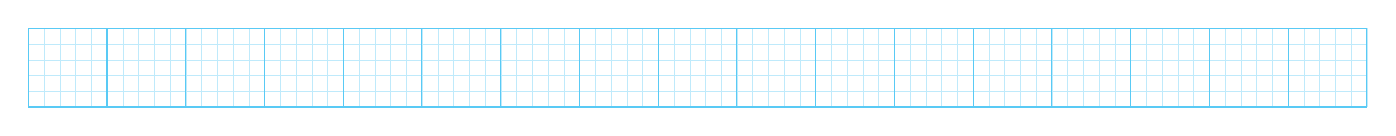
\begin{tikzpicture}
				\draw[cyan!25,ultra thin,step=0.2] (0,0) grid +(17,1);
				\draw[cyan!65] (0,0) grid +(17,1);
			\end{tikzpicture}\\[-1.1pt]
		}
	\end{center}
	\else
	\noindent%
	\begin{center}
		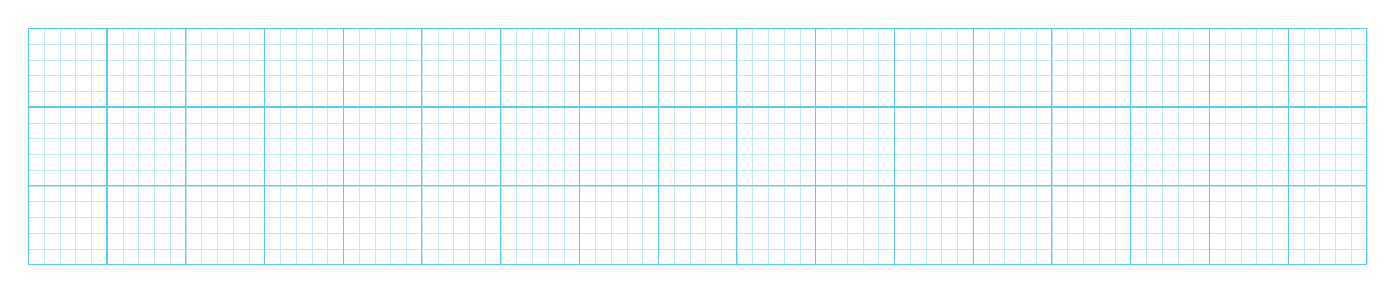
\begin{tikzpicture}
			\draw[cyan!25,ultra thin,step=0.2] (0,0) grid +(17,3);
			\draw[cyan!65] (0,0) grid +(17,3);
		\end{tikzpicture}
	\end{center}
	\fi
}

\def\Olyex{
	\AtBeginEnvironment{ex}{%
		\renewcommand{\loigiai}[1]{%
		\end{exbox}
		\def\exend{}
			\DoiThanhOly{##1}%
			\Writetofile{ansbook}{\string\def\string\writeANS{\saveans}}
			\scantokens{
				\begin{solbook}
					\writeANS
				\end{solbook}
			}		 
		}
	}
}
%%%=============================================%%%
\def\tatloigiaiex{%
\AtBeginEnvironment{ex}{\renewcommand{\loigiai}[1]{}}
}

%%%=============================================%%%
\def\hienthiloigiaiex{%
\AtBeginEnvironment{ex}{
\renewcommand{\loigiai}[1]{%
\end{exbox}
\def\exend{}
	\begin{center}
		{\color{\mycolor}\reflectbox{\Large\WritingHand}\ {\fmmfamily\LARGE Lời giải:}} 
	\end{center}
##1\hfill \faKey\ \circleTrue{\Alph{numTrue}} 
}
}
}

%%%=============================================%%%
\def\dongkebt{
\AtBeginEnvironment{bt}{
\renewcommand{\loigiai}[1]{
\end{btbox}
\def\btend{}
	\DoiThanhDongKe{##1}
}
}
}

%%%=============================================%%%
\def\dongkeHaicotbt{
\AtBeginEnvironment{bt}{
\renewcommand{\loigiai}[1]{
\end{btbox}
\def\btend{}
	\begin{multicols}{2}			
		\DoiThanhDongKeH{##1}
	\end{multicols}
}
}
}

%%%=============================================%%%
\def\tatloigiaibt{%
\AtBeginEnvironment{bt}{\renewcommand{\loigiai}[1]{}}
}

%%%=============================================%%%
\def\hienthiloigiaibt{%
\AtBeginEnvironment{bt}{
\renewcommand{\loigiai}[1]{%
\end{btbox}
\def\btend{}
	\begin{center}
		{\color{\mycolor}\reflectbox{\Large\WritingHand}\ {\fmmfamily\LARGE Hướng dẫn giải:}}
	\end{center}
##1
}
}
}



%%%=============================================%%%
\def\dongkevd{
\AtBeginEnvironment{vd}{
\renewcommand{\loigiai}[1]{%
\end{vdbox}\def\vdend{}
\vspace*{-\baselineskip}
\DoiThanhDongKe{##1}
}
}%
\AtBeginEnvironment{vdex}{
\renewcommand{\loigiai}[1]{%	
\end{boxvd}%
\def\vdexend{}
\par\noindent
\DoiThanhDongKe{##1}
}
}
}

%%%=============================================%%%
\def\dongkeHaicotvd{
\AtBeginEnvironment{vd}{
\renewcommand{\loigiai}[1]{%
\end{vdbox}\def\vdend{}
\begin{multicols}{2}			
\DoiThanhDongKeH{##1}
\end{multicols}
}
}%
\AtBeginEnvironment{vdex}{
\renewcommand{\loigiai}[1]{%	
\end{vdbox}%
\def\vdexend{}
\begin{multicols}{2}			
\DoiThanhDongKeH{##1}
\end{multicols}				
}
}
}

%%%=============================================%%%
\def\tatloigiaivd{
\AtBeginEnvironment{vd}{
\renewcommand{\loigiai}[1]{}%
}%
\AtBeginEnvironment{vdex}{
\renewcommand{\loigiai}[1]{}%
}
}

\def\hienthiloigiaivd{
\AtBeginEnvironment{vd}{
\renewcommand{\loigiai}[1]{
\end{vdbox}
\def\vdend{}
\begin{center}
	{\color{\mycolor}\reflectbox{\Large\WritingHand}\ {\fmmfamily\LARGE Bài làm:}}
\end{center}
##1
}
}
}

%%%=======================================================%%%
\newbool{Ads}
\newbool{Bds}
\newbool{Cds}
\newbool{Dds}
\def\saveans{}
\makeatletter
\newcommand{\KiemtraA}{\@ifnextchar\True{\global\setbool{Ads}{true}\xdef\saveans{\saveans\string\TLdung{A}}}{\global\setbool{Ads}{false}\xdef\saveans{\saveans\string\TLsai{A}}}}
\newcommand{\KiemtraB}{\@ifnextchar\True{\global\setbool{Bds}{true}\xdef\saveans{\saveans\string\TLdung{B}}}{\global\setbool{Bds}{false}\xdef\saveans{\saveans\string\TLsai{B}}}}
\newcommand{\KiemtraC}{\@ifnextchar\True{\global\setbool{Cds}{true}\xdef\saveans{\saveans\string\TLdung{C}}}{\global\setbool{Cds}{false}\xdef\saveans{\saveans\string\TLsai{C}}}}
\newcommand{\KiemtraD}{\@ifnextchar\True{\global\setbool{Dds}{true}\xdef\saveans{\saveans\string\TLdung{D}}}{\global\setbool{Dds}{false}\xdef\saveans{\saveans\string\TLsai{D}}}}
\makeatother

\newcommand{\choiceTF}[5][1]{%
\def\saveans{}%
\ifnum#1=1
\begin{enumerate}[wide=0.65cm,label*=\circlenum{\Alph*},itemsep=-3pt,topsep=-4pt,leftmargin =0.65cm]
\item\textcolor{gray}{\rule[-3pt]{0.65cm}{0.65pt}} \KiemtraA#2\dotEX	
\item\textcolor{gray}{\rule[-3pt]{0.65cm}{0.65pt}} \KiemtraB#3\dotEX
\item\textcolor{gray}{\rule[-3pt]{0.65cm}{0.65pt}} \KiemtraC#4\dotEX
\item\textcolor{gray}{\rule[-3pt]{0.65cm}{0.65pt}} \KiemtraD#5\dotEX
\end{enumerate}
\else
\begin{multicols}{#1}
\begin{enumerate}[wide=0.65cm,label*=\circlenum{\Alph*},itemsep=-3pt,topsep=-4pt,leftmargin =0.65cm]
\item\textcolor{gray}{\rule[-3pt]{0.65cm}{0.65pt}} \KiemtraA#2\dotEX	
\item\textcolor{gray}{\rule[-3pt]{0.65cm}{0.65pt}} \KiemtraB#3\dotEX
\item\textcolor{gray}{\rule[-3pt]{0.65cm}{0.65pt}} \KiemtraC#4\dotEX
\item\textcolor{gray}{\rule[-3pt]{0.65cm}{0.65pt}} \KiemtraD#5\dotEX
\end{enumerate}
\end{multicols}	
\fi
}

\newcommand{\LGexTF}{
\AtBeginEnvironment{ex}{
\renewcommand{\loigiai}[1]{%
\end{exbox}
\def\exend{}
\par\noindent%
{\reflectbox{\Large\WritingHand}\ {\fmmfamily\LARGE Hướng dẫn giải.}} ##1 \hfill{{\faKey}~ 
\ifbool{Ads}{\TLdung{A}}{\TLsai{A}}~
\ifbool{Bds}{\TLdung{B}}{\TLsai{B}}~
\ifbool{Cds}{\TLdung{C}}{\TLsai{C}}~
\ifbool{Dds}{\TLdung{D}}{\TLsai{D}} 
}%
\Writetofile{ansbook}{\string\def\string\writeANS{\saveans}}
\scantokens{
\begin{solbook}
\writeANS
\end{solbook}%
}%		
}
}
}
\newcommand{\LGbtTF}{
\AtBeginEnvironment{bt}{
\renewcommand{\loigiai}[1]{%
\par\noindent%
\end{btbox}
\def\btend{}
\par\noindent%
{\reflectbox{\Large\WritingHand}\ {\fmmfamily\LARGE Hướng dẫn giải.}} ##1 \hfill{{\faKey}~ 
\ifbool{Ads}{\TLdung{A}}{\TLsai{A}}~
\ifbool{Bds}{\TLdung{B}}{\TLsai{B}}~
\ifbool{Cds}{\TLdung{C}}{\TLsai{C}}~
\ifbool{Dds}{\TLdung{D}}{\TLsai{D}} 
}
}
}
}

\newcommand{\LGvdTF}{
\AtBeginEnvironment{vd}{
\renewcommand{\loigiai}[1]{%
\end{vdbox}
\def\vdend{}
\par\noindent%
{\reflectbox{\color{\mycolor}\Large\WritingHand}\ {\color{\mycolor}\fmmfamily\LARGE Lời giải.}} ##1 \hfill{{\faKey}~ 
\ifbool{Ads}{\TLdung{A}}{\TLsai{A}}~
\ifbool{Bds}{\TLdung{B}}{\TLsai{B}}~
\ifbool{Cds}{\TLdung{C}}{\TLsai{C}}~
\ifbool{Dds}{\TLdung{D}}{\TLsai{D}} 
}
}
}
}

\newcommand{\LGTNVD}{
\AtBeginEnvironment{vdex}{
\renewcommand{\loigiai}[1]{
\end{vdexbox}
\def\vdexend{}
\par\noindent{\color{\mycolor}\reflectbox{\Large\WritingHand}\ {\color{\mycolor}\fmmfamily\LARGE Lời giải.}}
##1\hfill\faKey\circlenum{\Alph{numTrue}} 
}
}
}
%%%=============================================%%%
\def\Olybt{
	\AtBeginEnvironment{bt}{
		\renewcommand{\loigiai}[1]{%
		\end{btbox}
		\def\btend{}
			\DoiThanhOly{##1}%		 
		}
	}
}

%%%=============================================%%%
\newcommand{\dienkhuyetLGBT}{
\AtBeginEnvironment{bt}{
\renewcommand{\loigiai}[1]{
\end{btbox}
\def\btend{}
\begin{center}
\begin{tikzpicture}[cyan!85!blue,opacity=0.55,thick,x=0.65cm,y=0.65cm]
\foreach \i in {14,...,22}{\draw (\i,0)--(\i,1);}
\draw[rounded corners=2pt] (13,0) rectangle (23,1);
\draw[rounded corners=2pt] (0,0) rectangle (11,1);
\path (0.25,0.5) node[anchor=west,font=\sffamily]{\color{\mycolor}\reflectbox{\Large\WritingHand}};
\end{tikzpicture}
\end{center}%\vspace*{-\baselineskip}
{\color{\mycolor}\reflectbox{\Large\WritingHand}\ {\fmmfamily\LARGE Hướng dẫn giải.}} ##1
}
}
}
%%%========================================%%%

\newcommand{\TLdung}[1]{%
\tikz[baseline=(char.base)]
{\node[shape=circle,inner sep=0.5pt,draw=\mauphu!90!cyan,%fill=#1!10,
font=\bfseries\footnotesize,text=\maudam,minimum size=12pt,outer sep=0pt] (char) {#1};
\path (char) node[text=\mauphu!90!cyan,opacity=0.65]{\faCheck};
}\ignorespaces}

\newcommand{\TLsai}[1]{%
\tikz[baseline=(char.base)]
{\node[shape=circle,inner sep=0.5pt,draw=\maunhan!30!red,font=\bfseries\footnotesize,minimum size=12pt,outer sep=0pt] (char) {#1};
\path (char) node[text=\maunhan!30!red,opacity=0.65]{\faTimes};
}\ignorespaces}
\def\saveans{}
\def\writeANS{}
\renewenvironment{Solbook}[1]{\noindent\textbf{\textsf{Câu~#1}}~}{ }
